% !Rnw root = ../diss.Rnw
\tikzstyle{element}=[rectangle, thick,
                     inner sep=0.1cm, rounded corners]
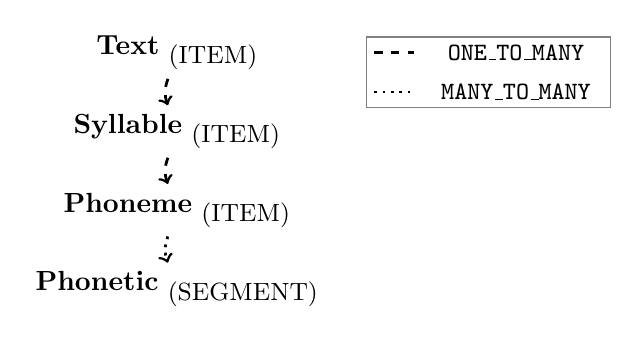
\begin{tikzpicture}
  
  %%%%%%%%%%%%%%%%%%%%%%%%%%%%%%
  %%%%%%%%%%%%%%%%%%%%%%%%%%%%%%
  % hierarchy

  %%%%%%%%%%%%%%%%%%%%%%%%%%%%%%
  % nodes
  % simple
  \node (text) at (0, 9) [element] {\textbf{Text} \textsubscript{\small{(ITEM)}}};

  \node (syl) at (0, 8) [element] {\textbf{Syllable} \textsubscript{\small{(ITEM)}}};
  
  \node (phoneme) at (0, 7) [element] {\textbf{Phoneme} \textsubscript{\small{(ITEM)}}};
  
  \node (phonetic) at (0, 6) [element] {\textbf{Phonetic} \textsubscript{\small{(SEGMENT)}}};

  %%%%%%%%%%%%%%%%%%%%%%%%%%%%%%
  % legends
  % simple
  \draw[gray] (2.4, 9.2) rectangle (5.5, 8.3);
  \node (leg_simp_o2m) at (4.3, 9) [element] {\small{\texttt{ONE\_TO\_MANY}}};
  \node (leg_sim_m2m) at (4.3, 8.5) [element] {\small{\texttt{MANY\_TO\_MANY}}};
  \draw [-, line width=1, dashed] (2.5, 9) to (3.0, 9);
  \draw [-, line width=1, dotted] (2.5, 8.5) to (3.0, 8.5);


  %%%%%%%%%%%%%%%%%%%%%%%%%%%%%%
  % links
  % simple
  \draw [->, line width=1, dashed] (text) to [bend right=20] (syl);

  \draw [->, line width=1, dashed] (syl) to [bend right=20] (phoneme);

  \draw [->, line width=1, dotted] (phoneme) to [bend right=20] (phonetic);


  
\end{tikzpicture}
